\section{Previous design}\label{sec:prev-design-analysis}
To test the hypothesised issue with the previous design, animations of the 2D simulation were produced and the change in mass of the solid phase was recorded.~\autoref{fig:old-design-phase-density} presents a screenshot at 2 seconds into the transient simulation. 
\begin{figure}[htbp]
    \centering
    
    \begin{minipage}{0.4\textwidth}
        \centering
        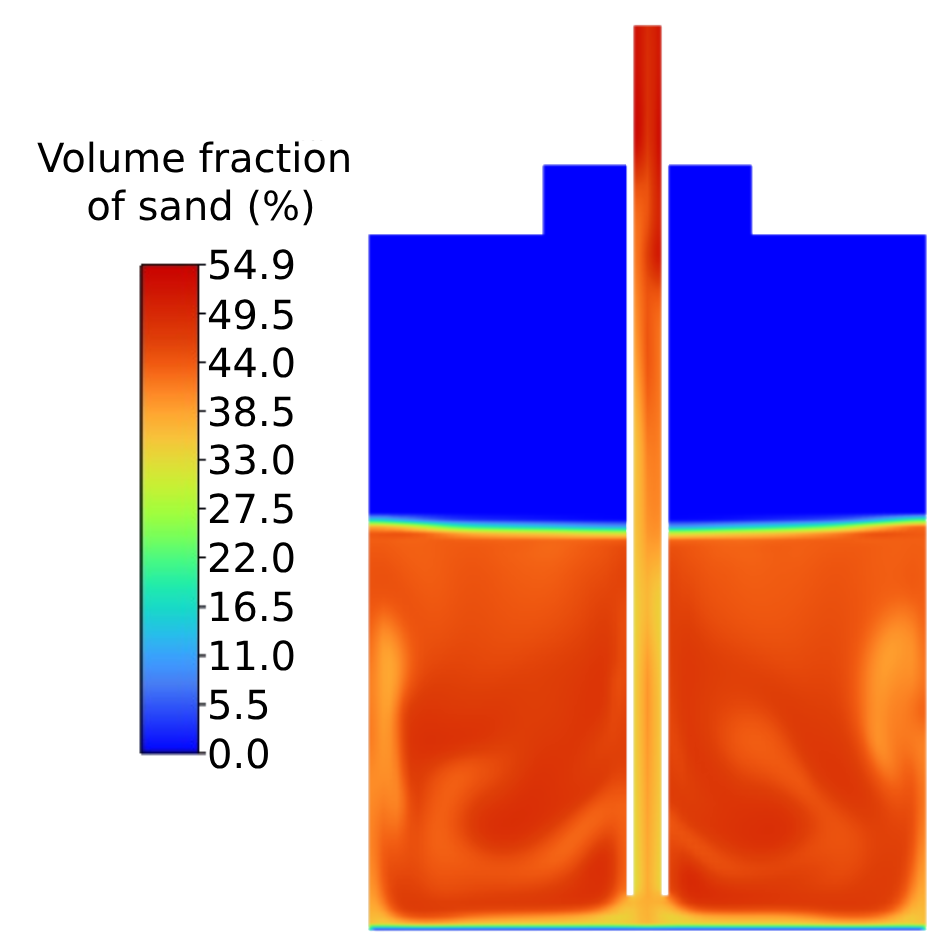
\includegraphics[width=\textwidth]{../report_assets/grav_better.png}
        \caption*{(a) Under Earth's Gravity}
    \end{minipage}
    \hfill
    \begin{minipage}{0.4\textwidth}
        \centering
        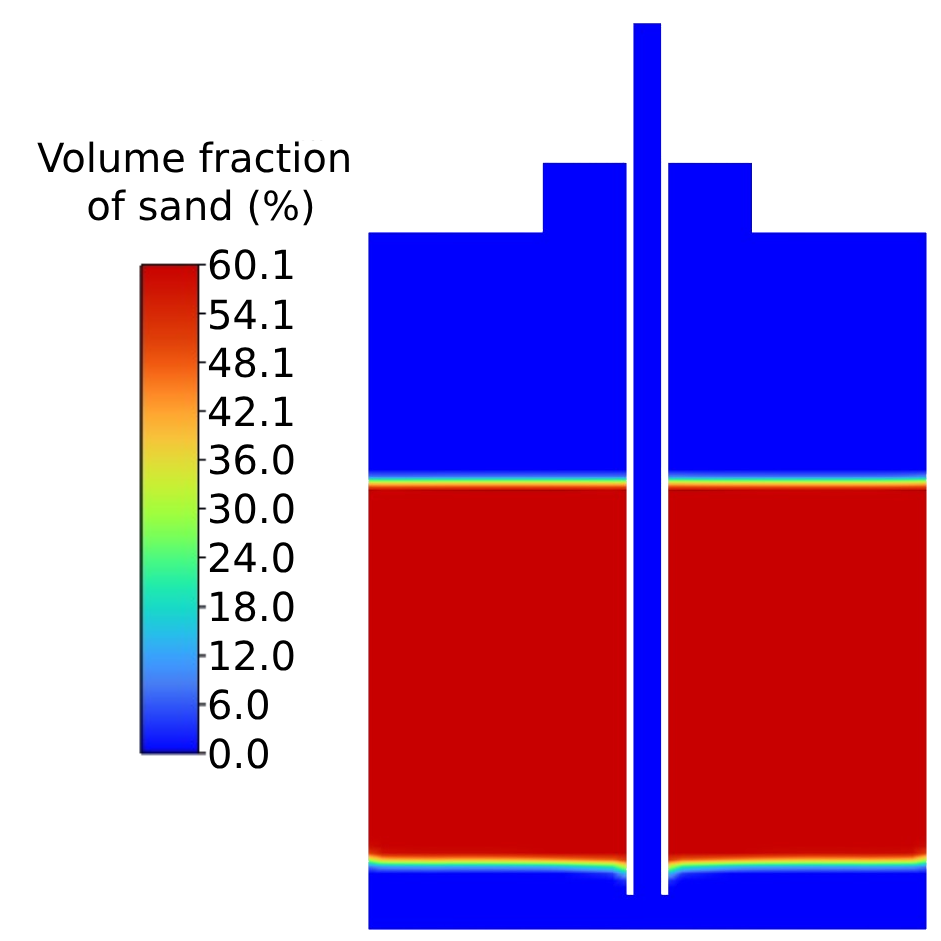
\includegraphics[width=\textwidth]{../report_assets/no_grav_better.png}
        \caption*{(b) Under Microgravity}
    \end{minipage}
    \caption{Phase Density of Old Design after 2 Seconds}\label{fig:old-design-phase-density}
\end{figure}
As shown, there is a marked difference in the location of powder between the two cases. While the powder in the tank under gravity appears to be fully fluidising, the tank in mircogravity is relatively unaffected by the flow. It is thought this is because the steady state flow does not interact with the region of the tank where the powder sits. For rigor, the unprocessed images are provided in \autoref{sec:unprocessed-images}.

\begin{figure}[htbp]
    \centering
    
    \begin{minipage}{0.54\textwidth}
        \centering
        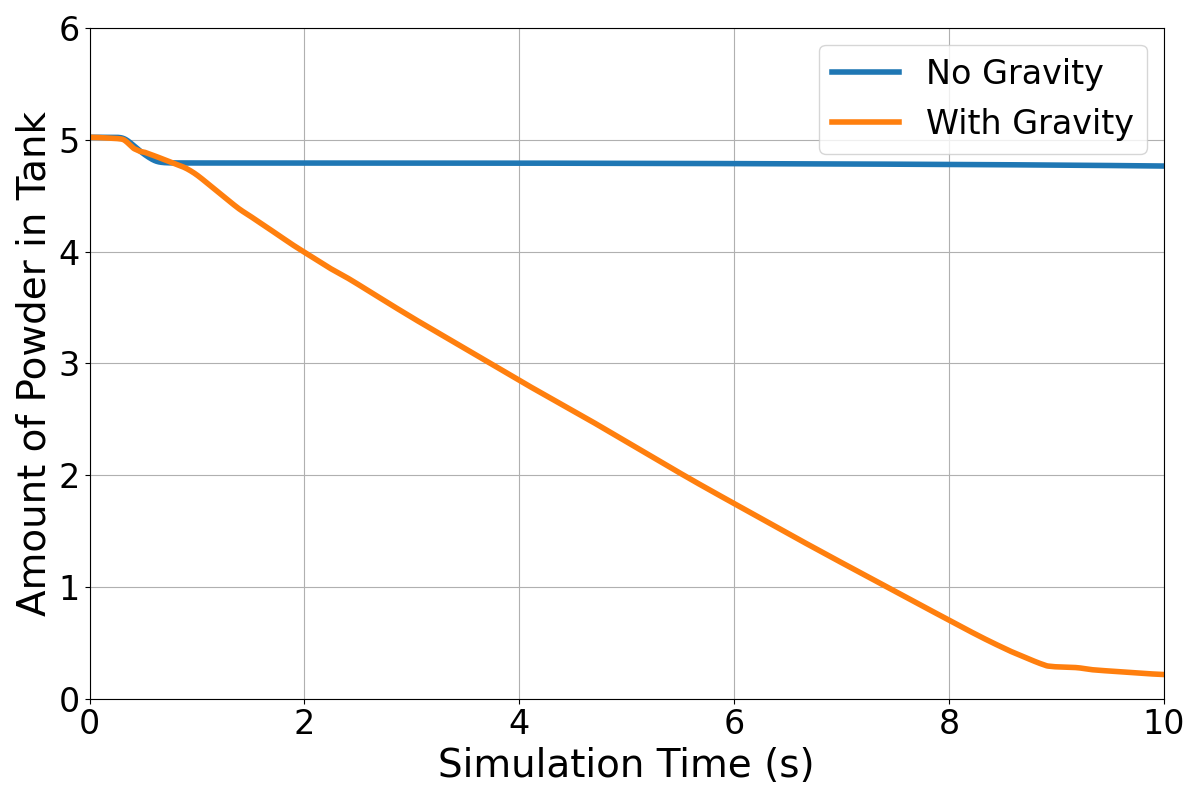
\includegraphics[width=\textwidth]{../report_assets/old_design_out.png}
        \caption{Change of Mass in the Tank Over Time}\label{fig:old-design-mass-change}
    \end{minipage}
    \hfill
    \begin{minipage}{0.4\textwidth}
        \centering
        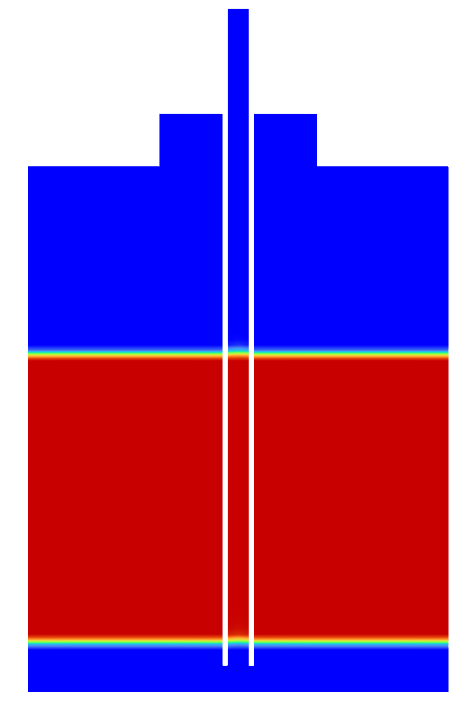
\includegraphics[width=0.6\textwidth]{../report_assets/old_initial.png}
        \caption{Initial Powder Configuration}\label{fig:old-initial}
    \end{minipage}
\end{figure}
\autoref{fig:old-design-mass-change} presents the amount of powder in the tank over time, measured by integrating the volume fraction of the solid phase over the entire geometry. At roughly 0.5s, both simulations show a relatively large drop in powder. This is because of how the simulation was initialised, shown in \autoref{fig:old-initial}, leading to the powder starting in the pipe quickly being expelled from the system. After this, there is a large gap between the two powder dispensing rates, again supporting the hypothesis that the previous design would be less appropriate for microgravity applications and supporting the decision to redesign the tank. 

As mentioned in \autoref{sec:old-design-method}, this analysis was conducted with a relatively coarse mesh which may alter the results. The biggest impact would be not resolving key gradients or incorrect momentum exchange between the two phases. As this geometry is relatively simplistic and the velocity into the system small, it is assumed that there would be minimal impact from not resolving velocity or pressure gradients well enough. However, it is less clear how accurately the momentum exchange is affected by this and was assumed to be valid just based off the authors understanding of the expected behaviour of the system. Given more time this would be an area of focus, conducting a mesh convergence study and running the finer meshes for a longer time should be done to validate this preliminary result. Another area for improvement is using an inlet condition more accurate to the physics. A pressure inlet would have been ideal as this is closer to the physics of the system but due to limitations of the simulation software, there was no way to prevent the powder exiting this inlet. This could be fixed with a user defined function, found through simulating the system with a pressure inlet and no powder, and then transferred to this analysis.
\section{Characterising Pressure Source}\label{sec:static_test}
\subsection{Initial Test}
The first step in characterising the system was to investigate the static pressure losses present in the tank without a piston or any powder. This immediately presented a problem as the static pressure readings, given a gas source with a stagnation pressure of 4 to 6 bar, were far below expected, as seen in figure \autoref{fig:static-pressure-drop}. 
\begin{figure}[htbp]
    \centering

    \begin{minipage}{0.45\textwidth}
        \centering
        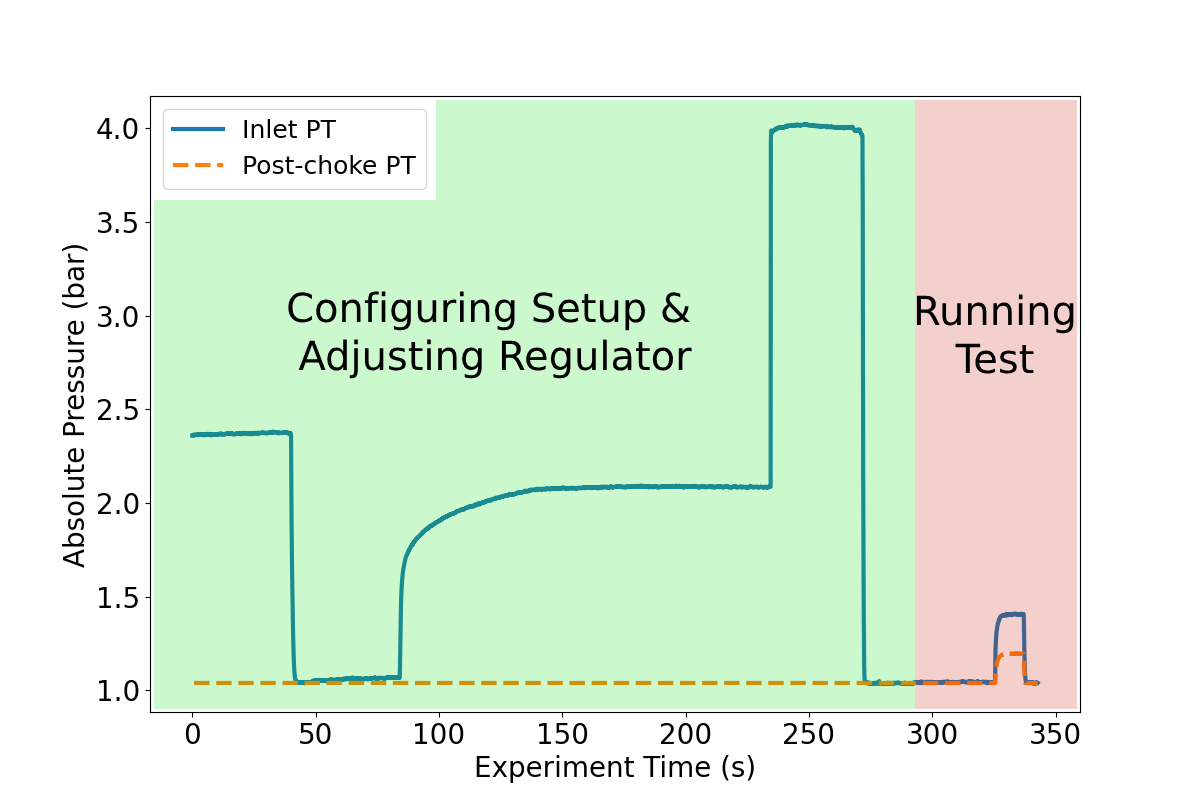
\includegraphics[width=\textwidth]{../report_assets/3_bar_static_full.png}
        \caption*{(a) Full 4 bar test.}
    \end{minipage}
    \hfill
    \begin{minipage}{0.45\textwidth}
        \centering
        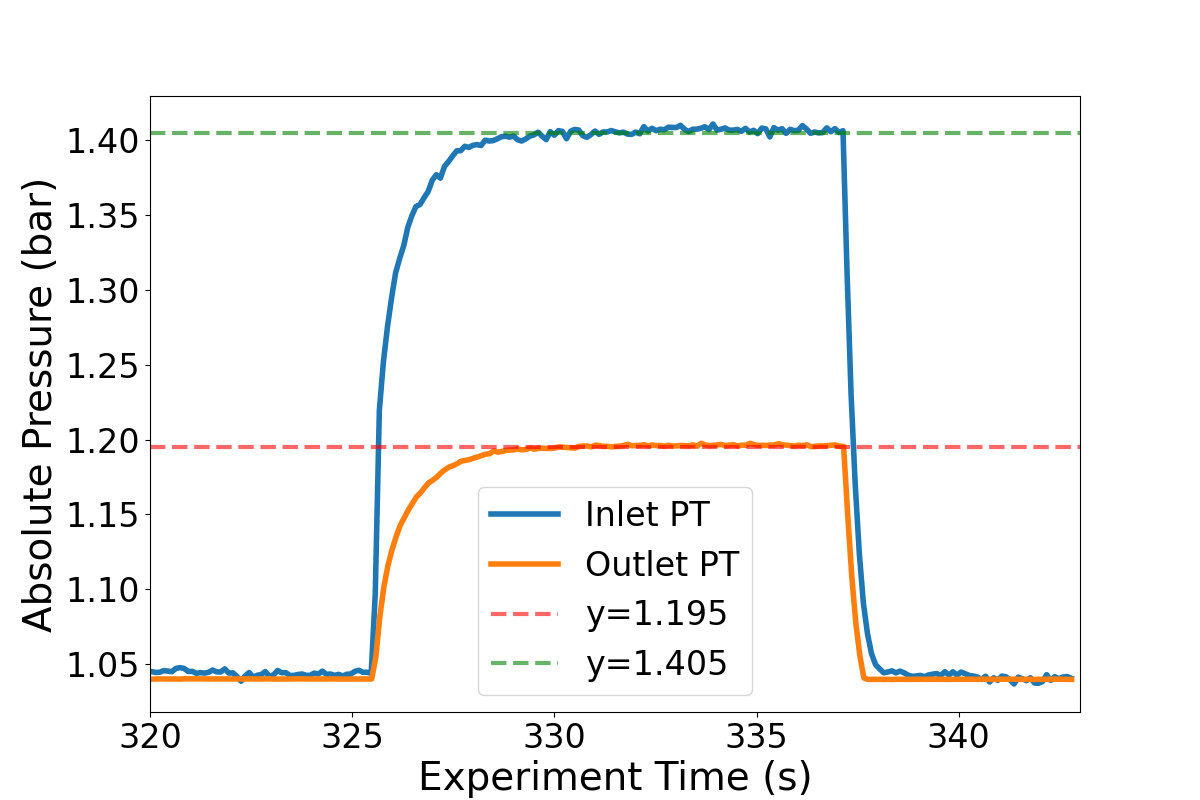
\includegraphics[width=\textwidth]{../report_assets/3_bar_static.png}
        \caption*{(b) Static pressure from 4 bar.}
    \end{minipage}
    \begin{minipage}{0.45\textwidth}
        \centering
        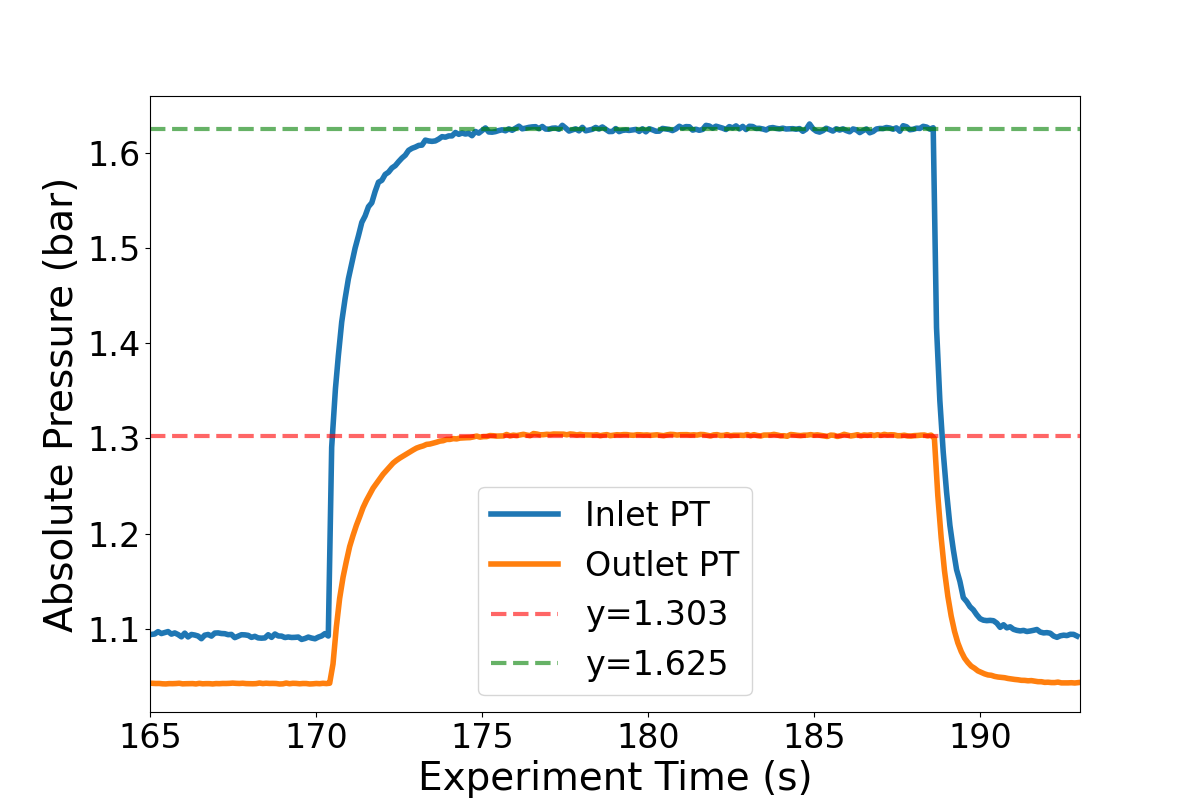
\includegraphics[width=\textwidth]{../report_assets/4_bar_static.png}
        \caption*{(c) Static pressure from 5 bar.}
    \end{minipage}
    \hfill
    \begin{minipage}{0.45\textwidth}
        \centering
        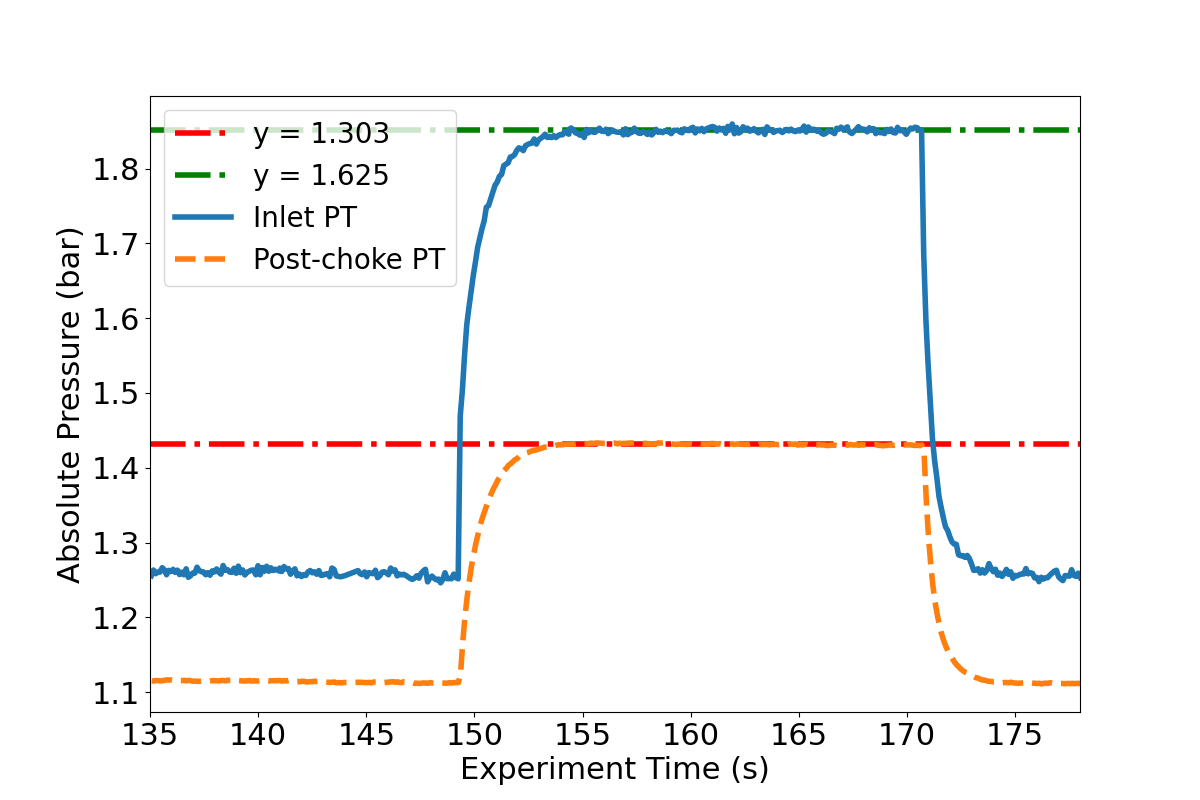
\includegraphics[width=\textwidth]{../report_assets/5_bar_static.png}
        \caption*{(d) Static pressure from 6 bar.}
    \end{minipage}

    \caption{Full caption mb?}\label{fig:static-pressure-drop}
\end{figure}
If the compressed air line was truely supplying a stagnation pressure of 4 bar, through isentropic flow relations the data implies that the mach number of the flow is 1.3 which is unlikely.

As seen in \autoref{fig:static-pressure-drop} (a), the regulator was able to control the static pressure to 4 bar when the system was closed. When the system opens, one could expect that the regulator would maintain this 4 bar static pressure and only static pressure losses in the system and acceleration of the flow beyond the regulator would reduce it somewhat. However, by the time the flow reached the pressure transducer before the tank, the static pressure had dropped to 1.4 bar. 

Assuming the flow was mach 1 through the nylon pipe, this would imply a stagnation pressure of roughly 2 bar not the 4 bar initially desired. As seen in~\autoref{fig:static-pressure-drop} (c) and (d), this behaviour was persistant at higher inlet pressures, dont really know why rn but justify when i do

\subsection{Further Investigation}
In an attempt to diagnose this behaviour, follow up tests were conducted. As seen in figure the performance was much worse giving even lower static pressure readings. 
\begin{figure}[htbp]
    \centering

    \begin{minipage}{0.45\textwidth}
        \centering
        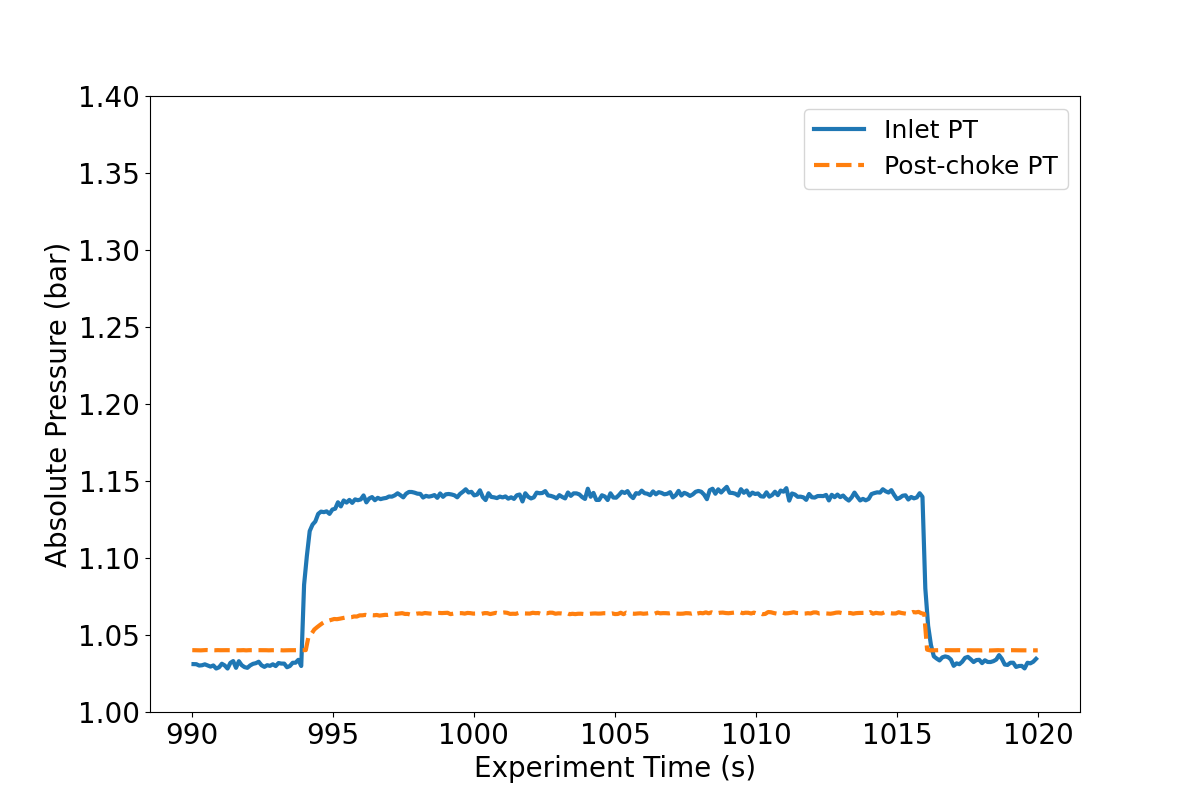
\includegraphics[width=\textwidth]{../report_assets/3_bar_static_new_reg.png}
        \caption{New regulator.}\label{fig:static-pressure-drop-new-reg}
    \end{minipage}
    \hfill
    \begin{minipage}{0.45\textwidth}
        \centering
        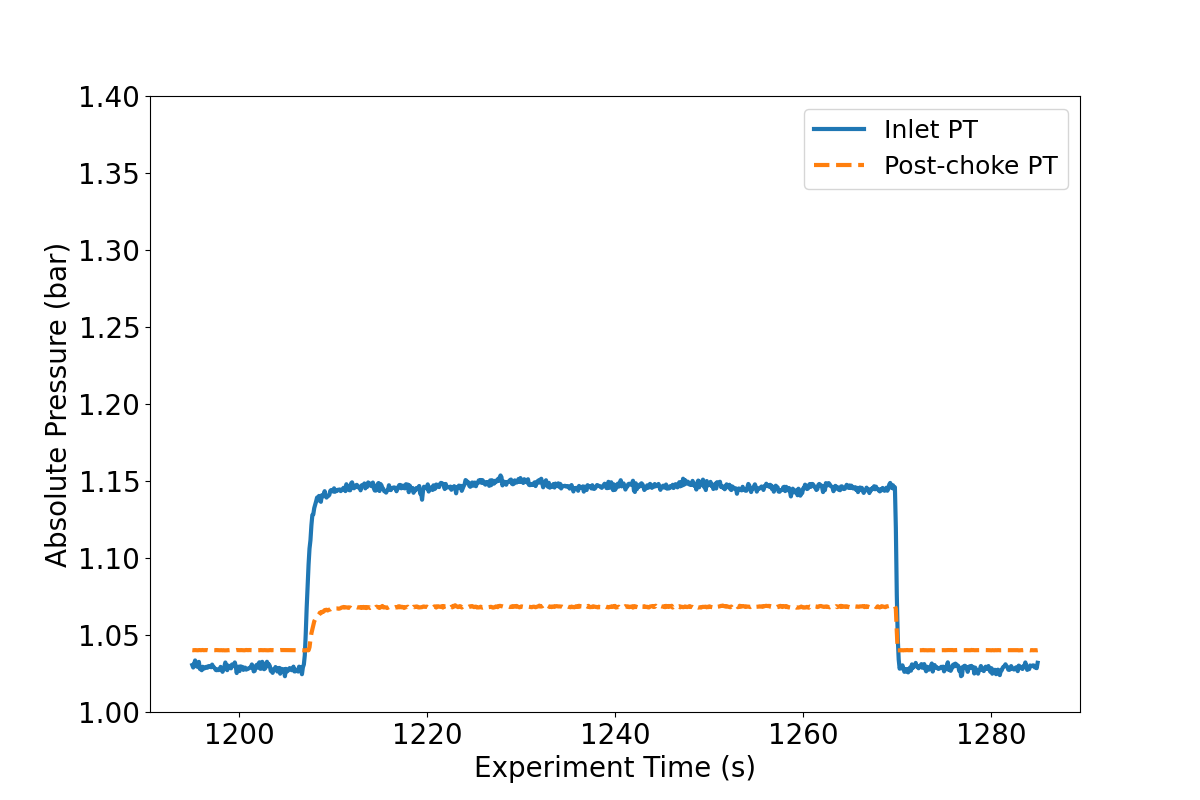
\includegraphics[width=\textwidth]{../report_assets/3_bar_static_no_solenoid.png}
        \caption{New regulator + no solenoid.}\label{fig:static-pressure-drop-no-solenoid}
    \end{minipage}

\end{figure}
As a final attempt, the solenoid valve was removed from the set up to verify that this wasnt choking the flow or somehow drastically decreasing static pressure somehow. Again, seen in fig 6, this performed similarly to the setup containing the regulator so wasn't the cause of the behaviour and the system diagram was reverted to \autoref{fig:systems-diagram}.

\subsection{Simulation}
A 2D Axisymmetric analysis of the empty tank was conducted using fluent. This seemed to support the idea that only 1bar of stagnation pressure was being supplied to the system, not the desired 3bar as setting the pressure inlet to 1bar gave comparable static pressure readings as seen in the tests.
\begin{figure}[htbp]
    \centering

    \begin{minipage}{0.45\textwidth}
        \centering
        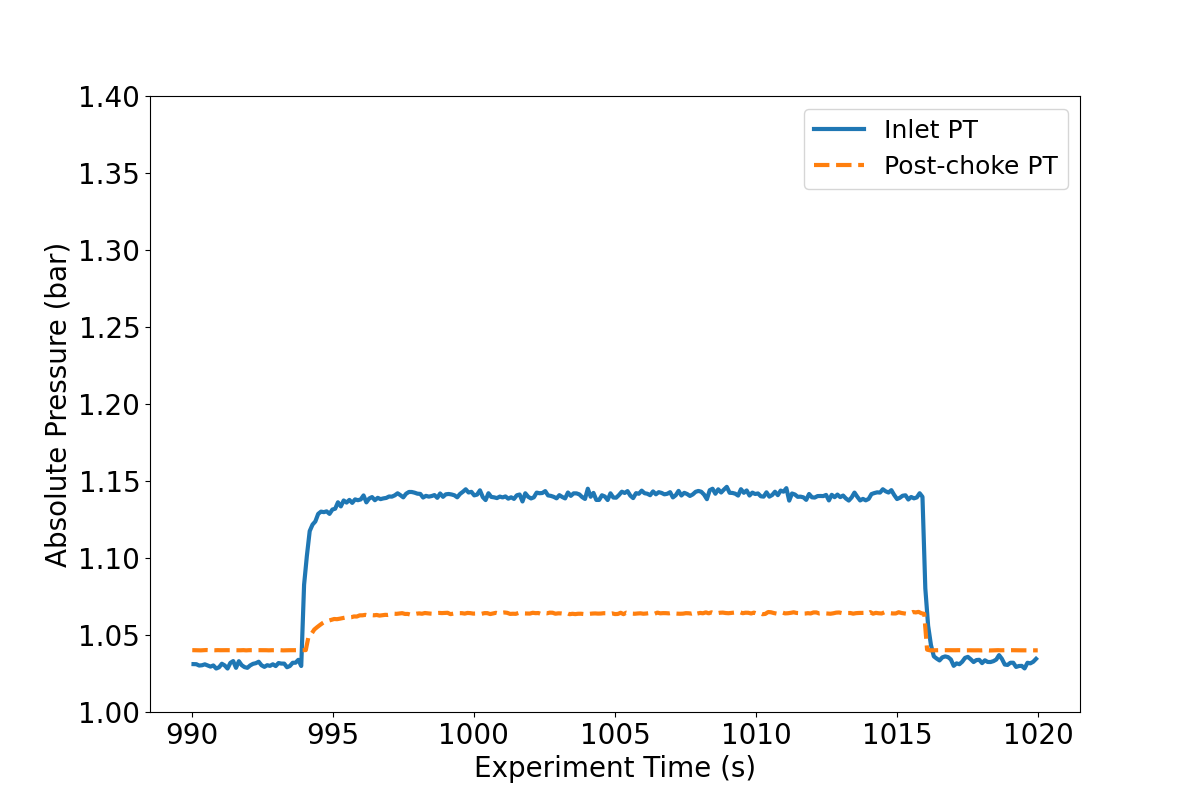
\includegraphics[width=\textwidth]{../report_assets/3_bar_static_new_reg.png}
        \caption{New regulator.}\label{fig:static-pressure-drop-fluent}
    \end{minipage}
    \hfill
    \begin{minipage}{0.45\textwidth}
        \centering
        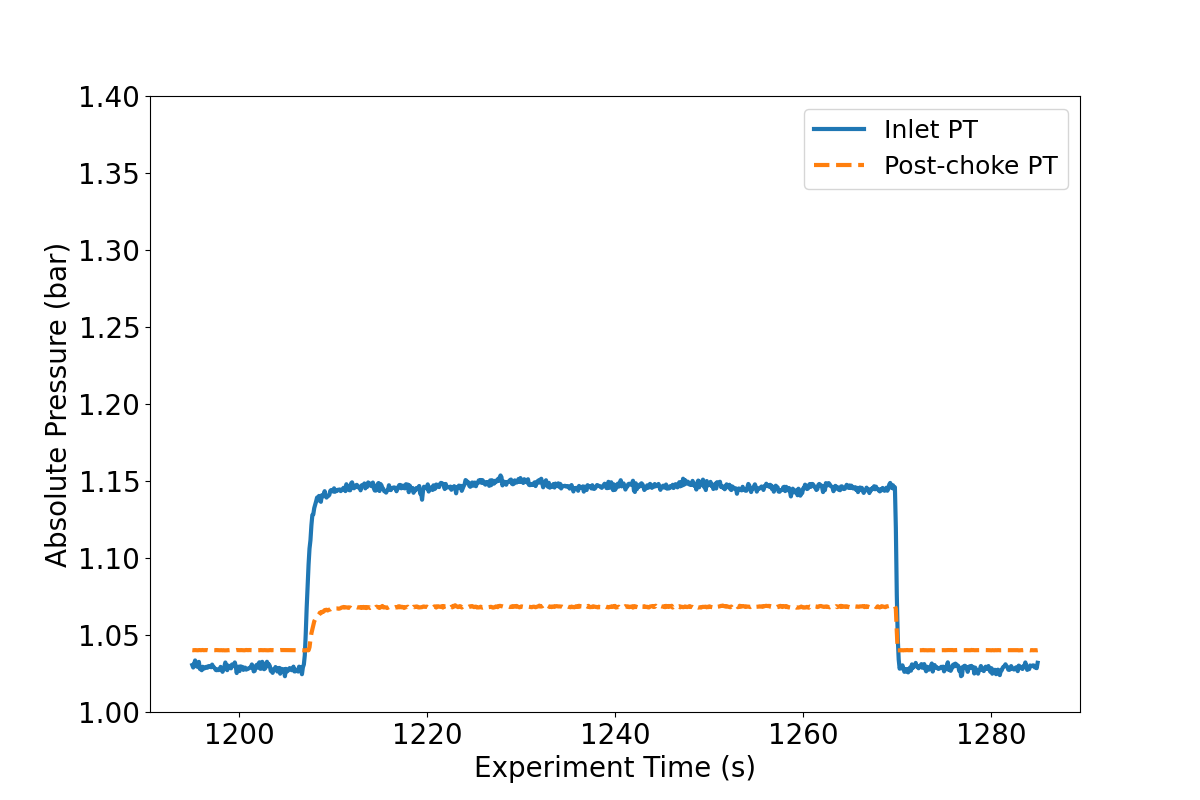
\includegraphics[width=\textwidth]{../report_assets/3_bar_static_no_solenoid.png}
        \caption{New regulator + no solenoid.}\label{fig:static-pressure-drop-report}
    \end{minipage}

\end{figure}

\subsection{Stagnation pressure values}
Given the unreliability of the pressure gauge, a number of assumptions were made to determine the stagnation pressure and allow for analysis of mass flow rate against pressure. Assuming that the flow was choked within the tubes, having a velocity of 343m/s, the isentropic relations give that p/p0 =  0.52828178
\begin{table}[htbp]
    \centering
    \begin{tabular}{|c|c|c|}
        \hline
        Pressure regulator setting (bar) & Static Pressure at inlet (bar) &  Stagnation Pressure (bar) \\
        \hline
        4 & 1.405 & 2.66 \\
        5 & 1.625 & 3.08 \\
        6 & 1.852 & 3.51 \\
        \hline
    \end{tabular}
    \caption{Summary of static and stagnation pressures for different tests.}
    \label{tab:static-stag-pressures}
\end{table}

\newpage
\section{First Test}\label{sec:first-test}
As mentioned in \autoref{sec:piston}, the very first test with was conducted without sand and failed to push the piston down the tank. This quick test was the motivation to characterise the pressure source as it was noted that the pressure readings before and after the tank were lower than expected and changed slower than expected. This meant that the failure mode of the piston crumpling was discounted and the future piston designs ignored this possibility. After characterisation of the pressure source, the second piston was tested, seen in \autoref{fig:first-test}. 

\begin{figure}[htbp]
    \centering
    
    \begin{minipage}{0.6\textwidth}
        \centering
        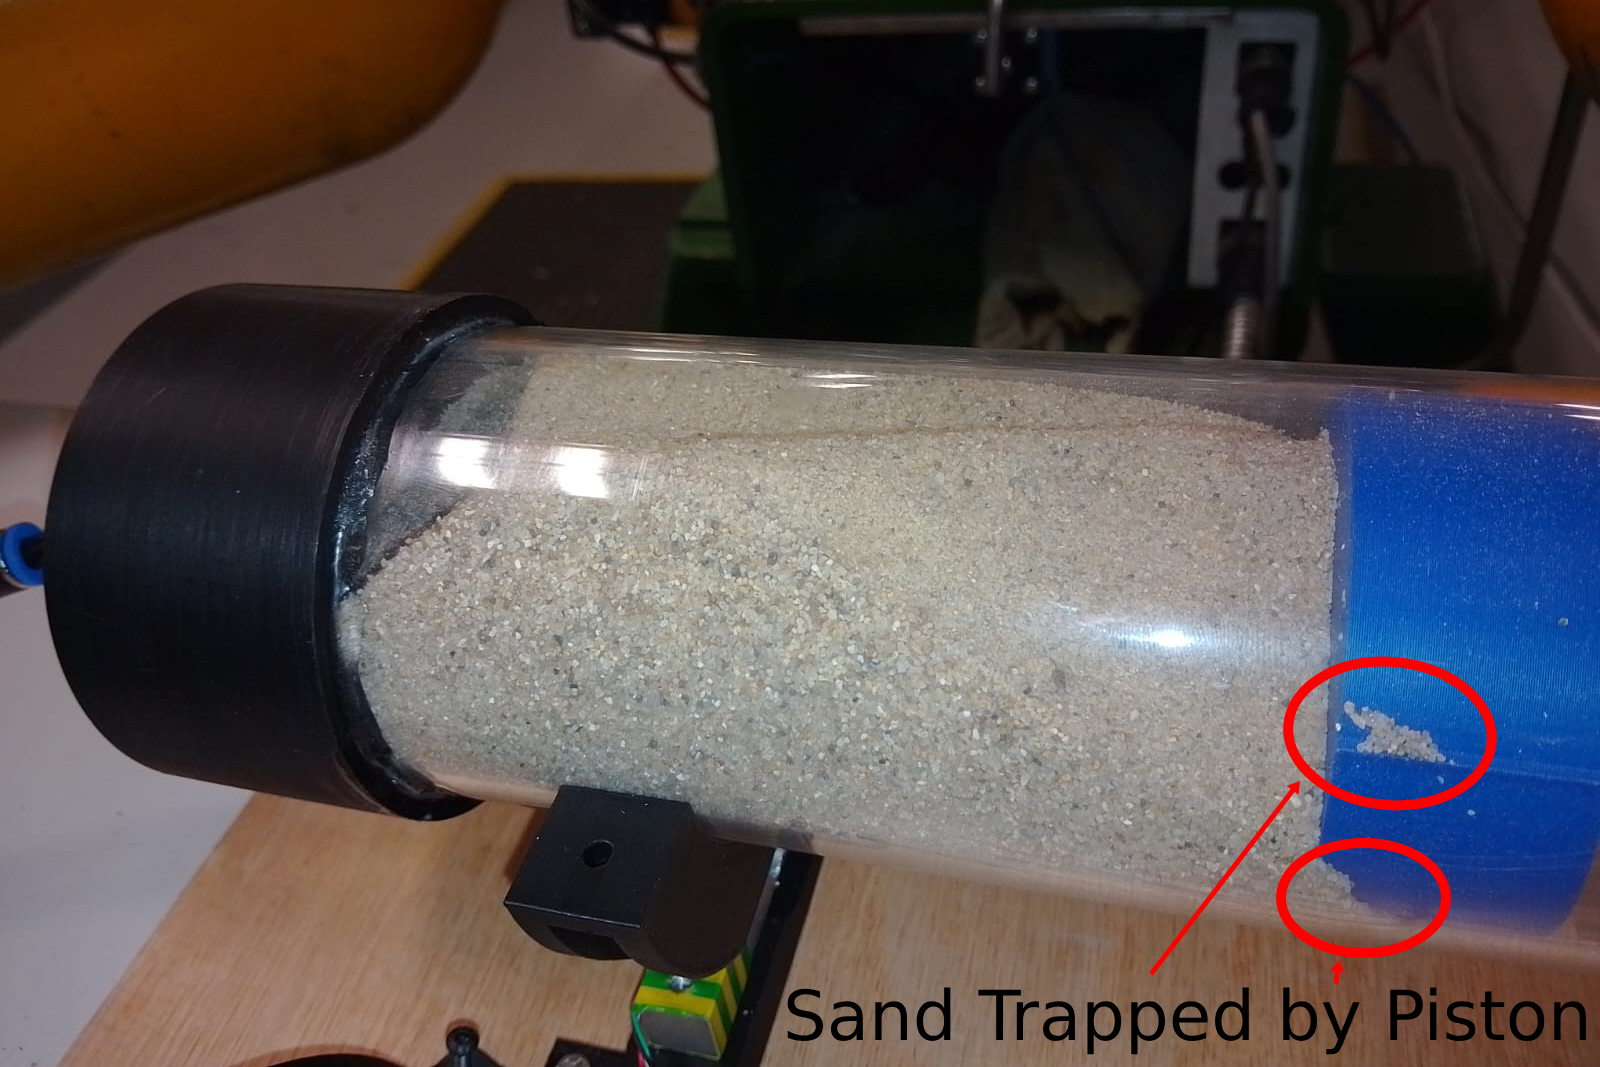
\includegraphics[width=\textwidth]{../report_assets/first_test.png}
        \caption{Result of First Powder Test}\label{fig:first-test}
    \end{minipage}
    
\end{figure}
The piston started far down the tank and was successfully pushed towards the outlet. At the point it reached the sand, it became stuck, as the unpacked grains formed a wedge under the piston and caused it to jam into the side walls of the tank. With the powder not compacted against the outlet, ratholing began to occur as the gas entrained the sand particles through the outlet, highlighting an alternate dispensing regime to be avoided. The gap between the piston and the walls was designed to be 1mm so it is expected that this specific issue would not have occured with a finer grain sand. While purchasing finer grain sand or crushing down the current sample were considered, it was decided that a new design would be investigated as this was not something seen in the literature and would be much easier to characterise the friction. A full analysis of the piston was of great interest but given the limited time of the project, was deemed out of the scope. 


\newpage
\section{Main Experiment}
\begin{figure}[htbp]
    \centering

    \begin{minipage}{0.3\textwidth}
        \centering
        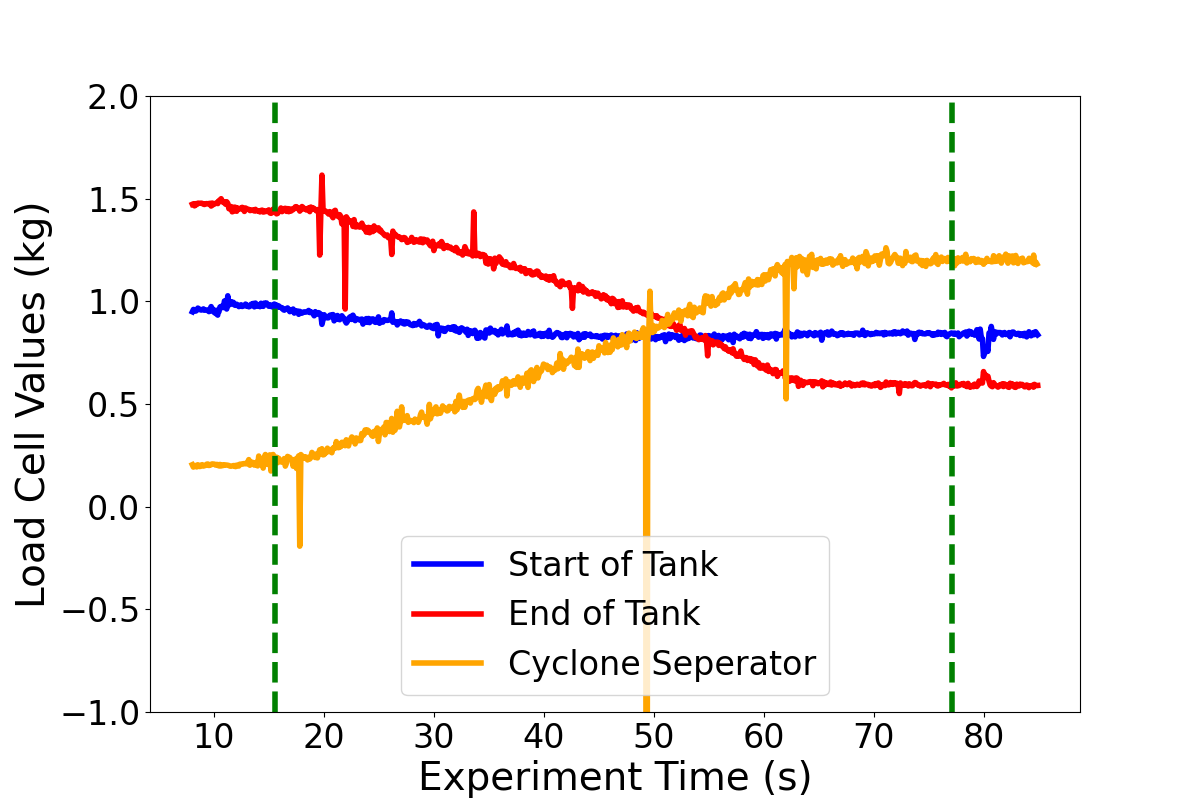
\includegraphics[width=\textwidth]{../report_assets/41_raw_mass.png}
        \caption*{Raw Load Cell Readings.}
    \end{minipage}
    \hfill
    \begin{minipage}{0.3\textwidth}
        \centering
        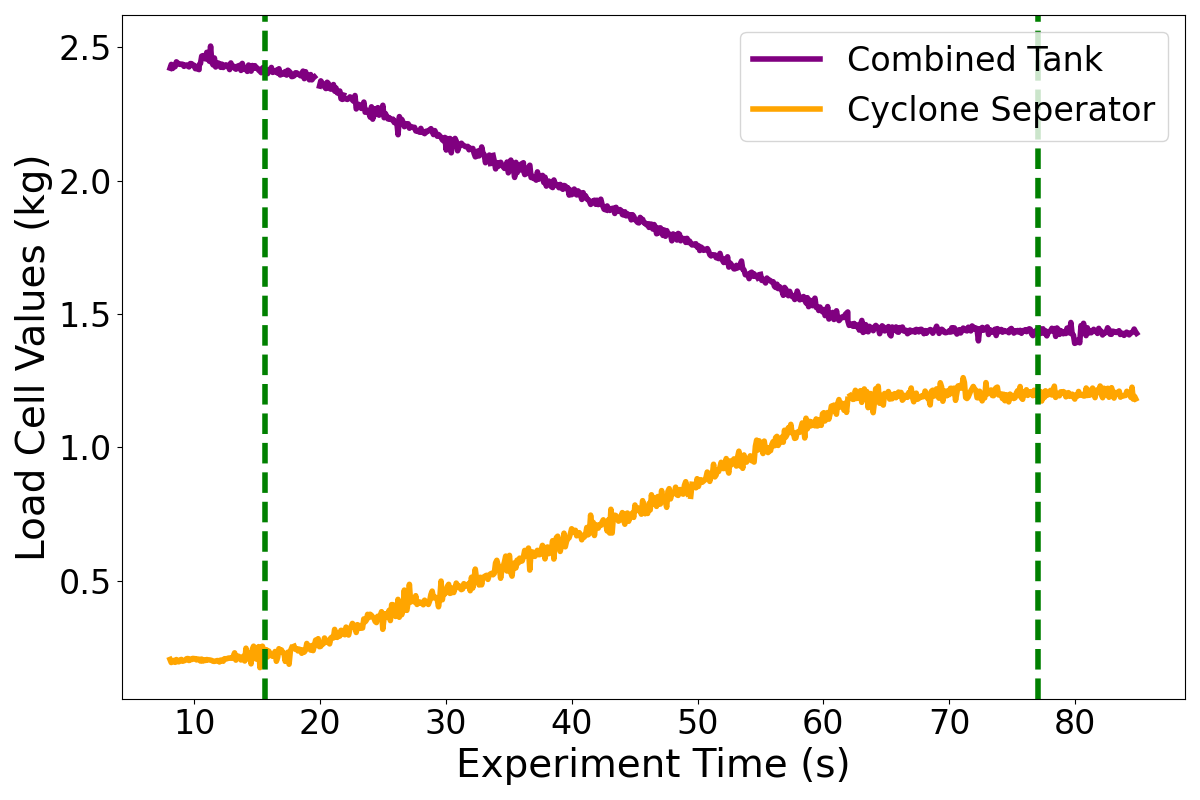
\includegraphics[width=\textwidth]{../report_assets/41_clean_mass.png}
        \caption*{Cleaned Mass Change.}
    \end{minipage}
    \hfill
    \begin{minipage}{0.3\textwidth}
        \centering
        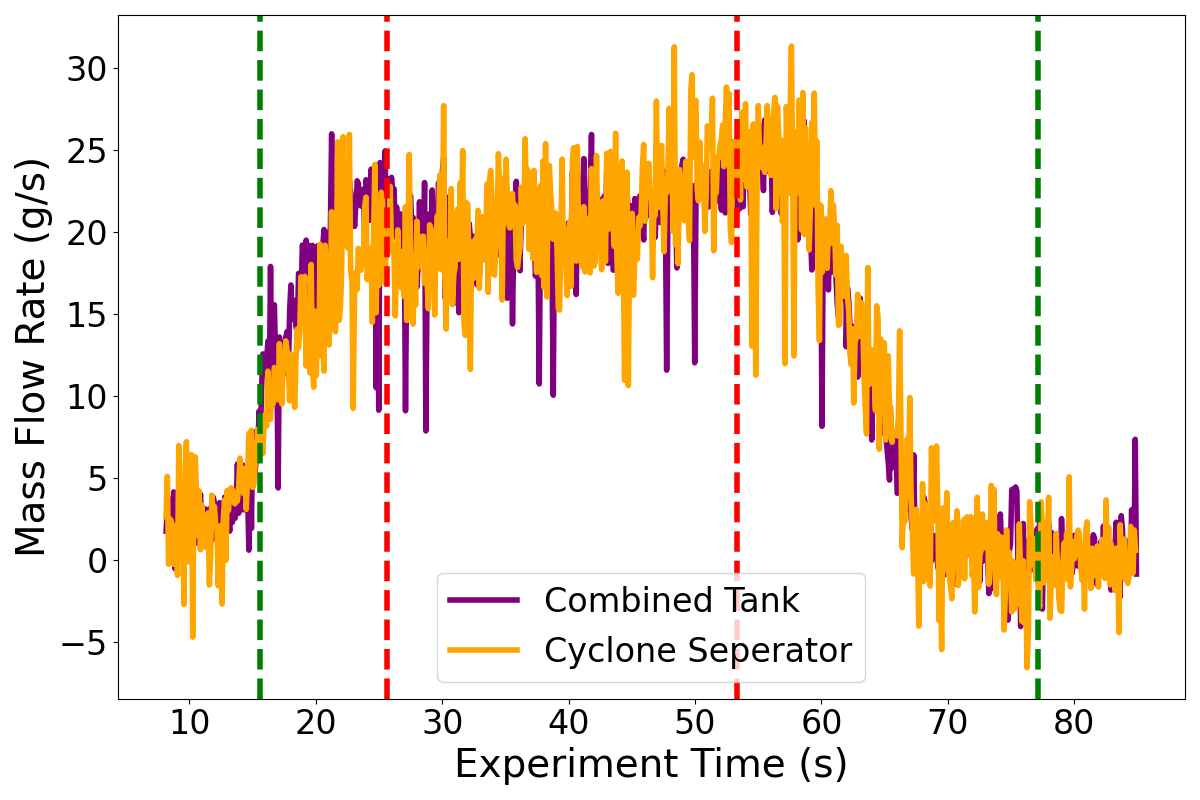
\includegraphics[width=\textwidth]{../report_assets/41_clean_flow_100.png}
        \caption*{Mass Flow Rate with 100 smoothing.}
    \end{minipage}
    \caption{1st Test 4 Bar Inlet}

\end{figure}\label{fig:41}

\begin{figure}[htbp]
    \centering

    \begin{minipage}{0.3\textwidth}
        \centering
        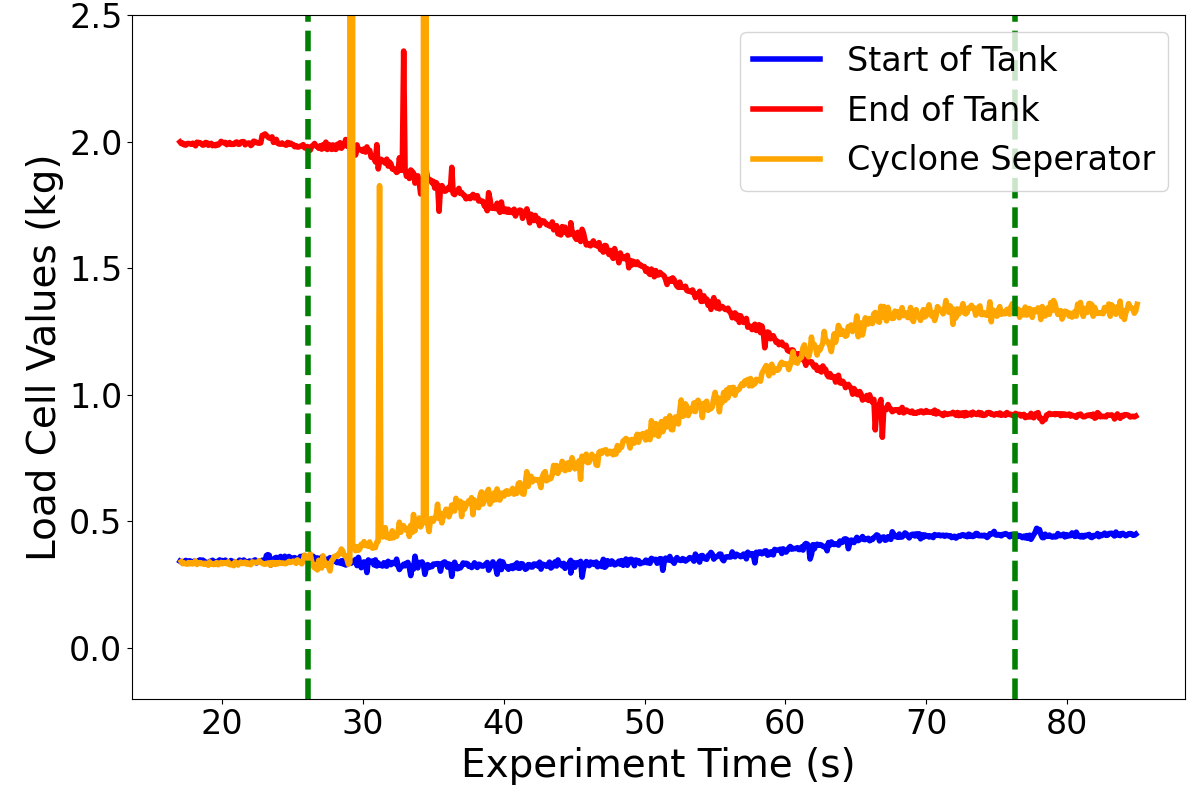
\includegraphics[width=\textwidth]{../report_assets/42_raw_mass.png}
        \caption*{Raw Load Cell Readings.}
    \end{minipage}
    \hfill
    \begin{minipage}{0.3\textwidth}
        \centering
        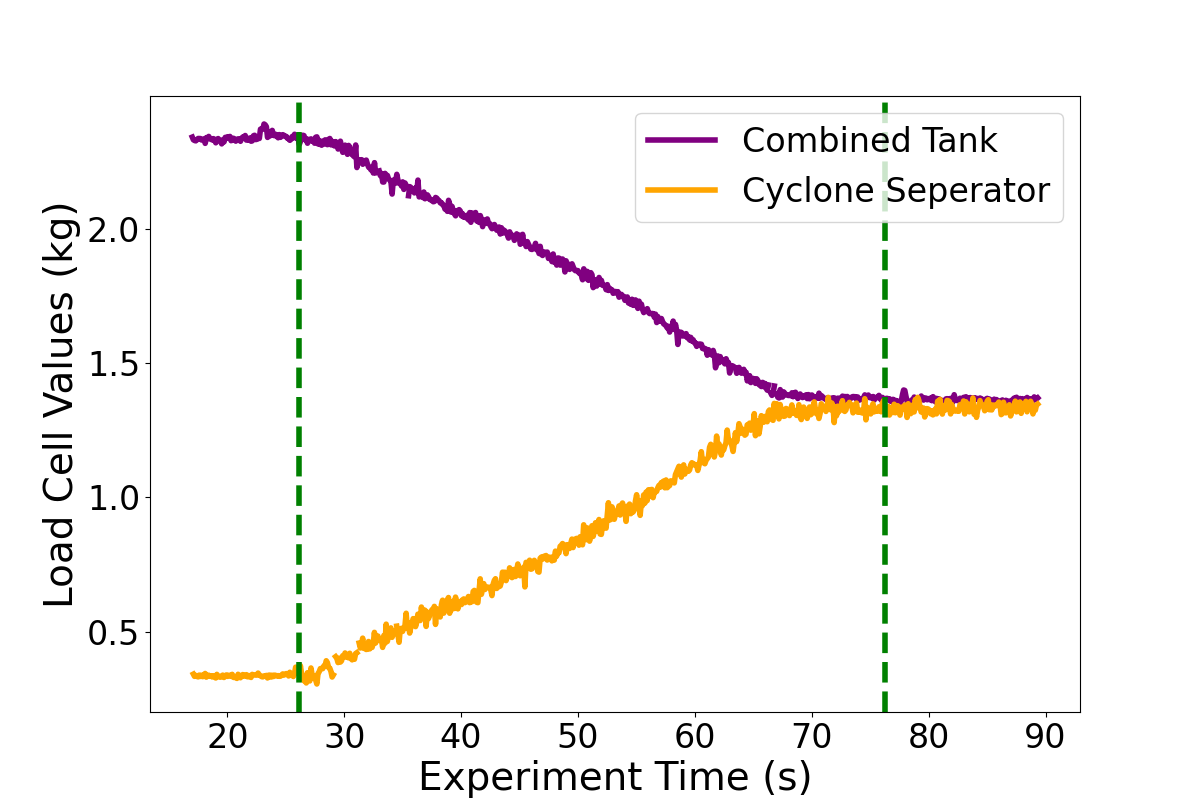
\includegraphics[width=\textwidth]{../report_assets/42_clean_mass.png}
        \caption*{Cleaned Mass Change.}
    \end{minipage}
    \hfill
    \begin{minipage}{0.3\textwidth}
        \centering
        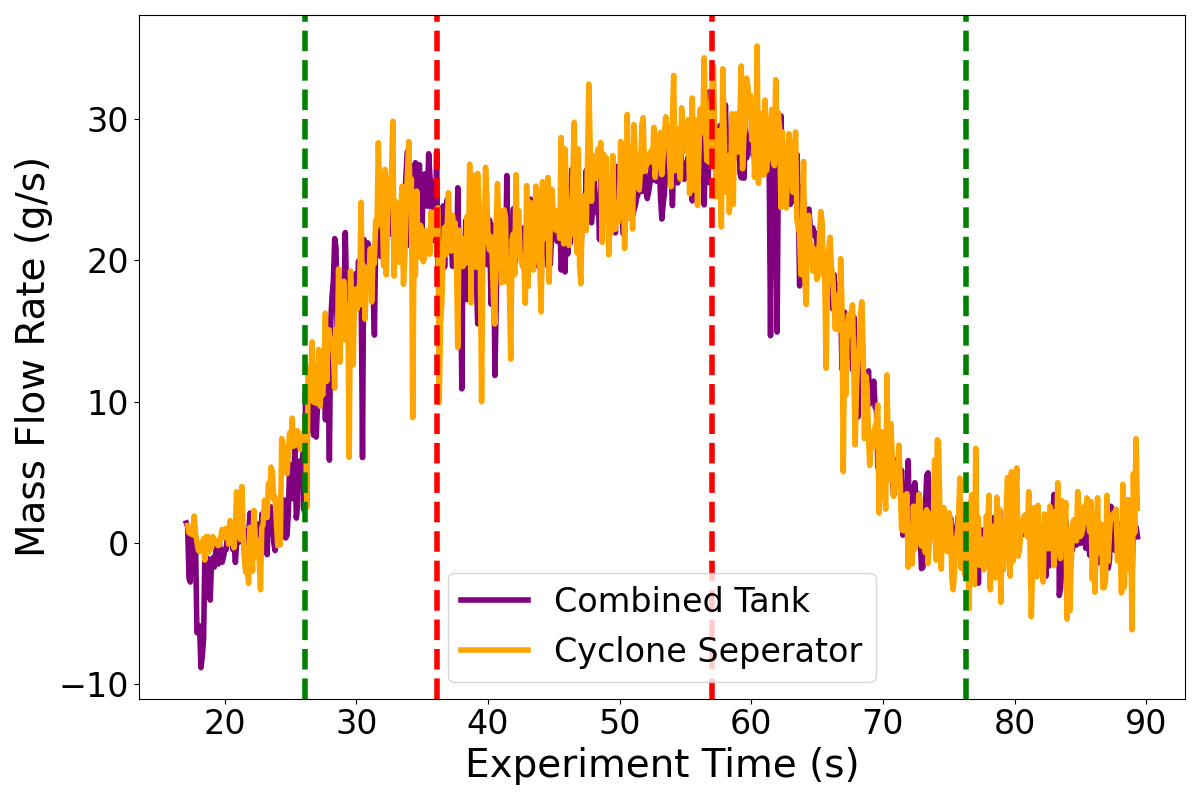
\includegraphics[width=\textwidth]{../report_assets/42_clean_flow_100.png}
        \caption*{Mass Flow Rate with 100 smoothing.}
    \end{minipage}
    \caption{2nd Test 4 Bar Inlet}
    
\end{figure}\label{fig:42}

\begin{figure}[htbp]
    \centering

    \begin{minipage}{0.3\textwidth}
        \centering
        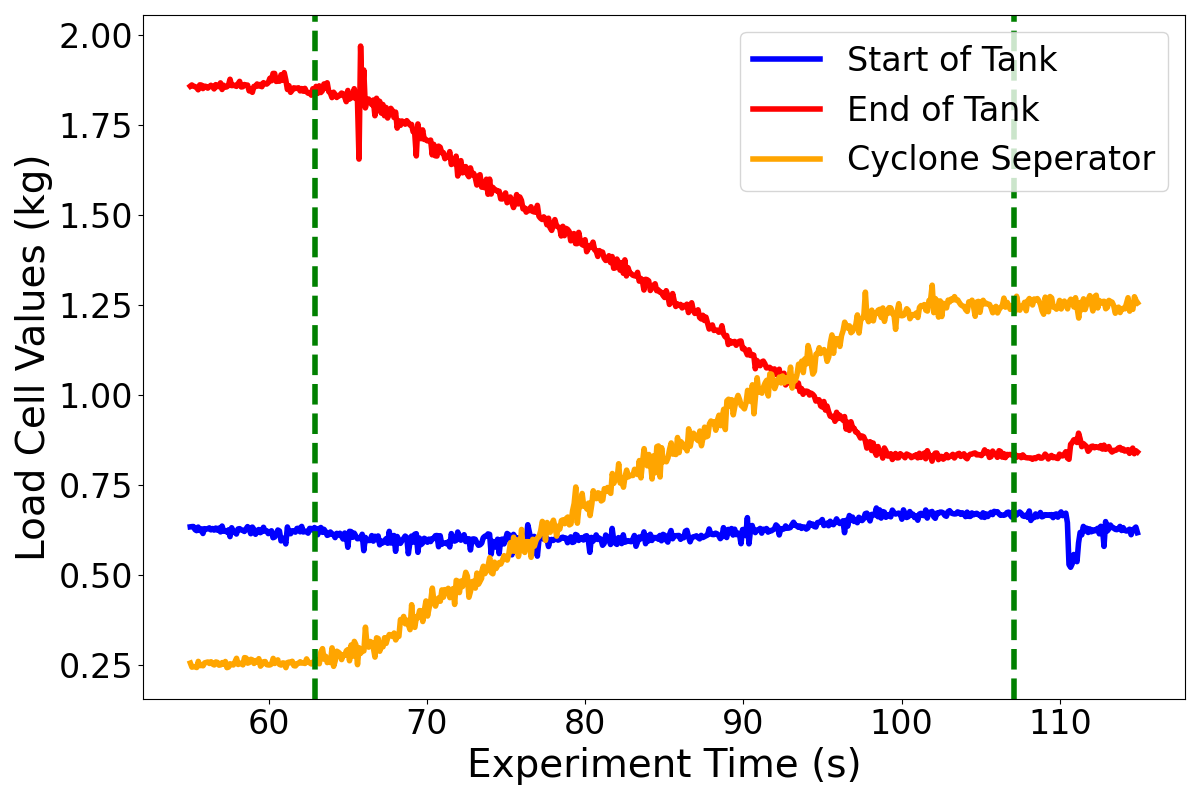
\includegraphics[width=\textwidth]{../report_assets/43_raw_mass.png}
        \caption*{Raw Load Cell Readings.}
    \end{minipage}
    \hfill
    \begin{minipage}{0.3\textwidth}
        \centering
        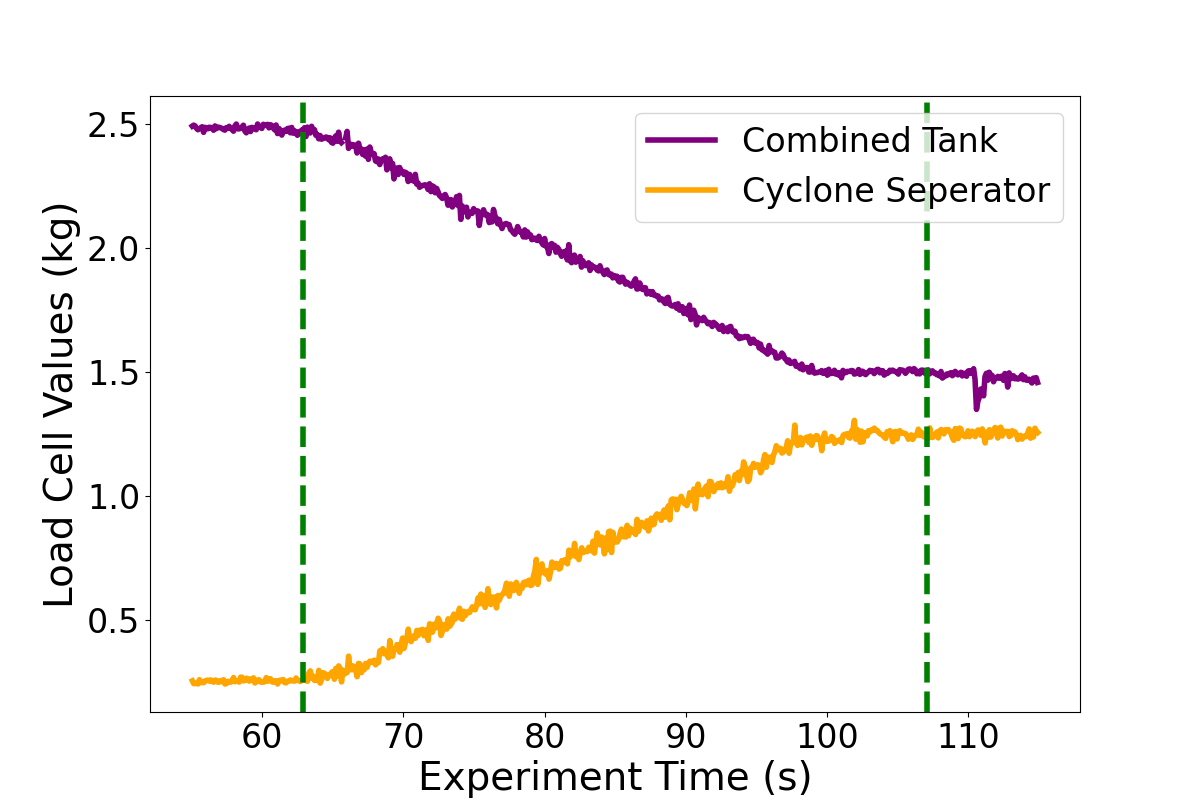
\includegraphics[width=\textwidth]{../report_assets/43_clean_mass.png}
        \caption*{Cleaned Mass Change.}
    \end{minipage}
    \hfill
    \begin{minipage}{0.3\textwidth}
        \centering
        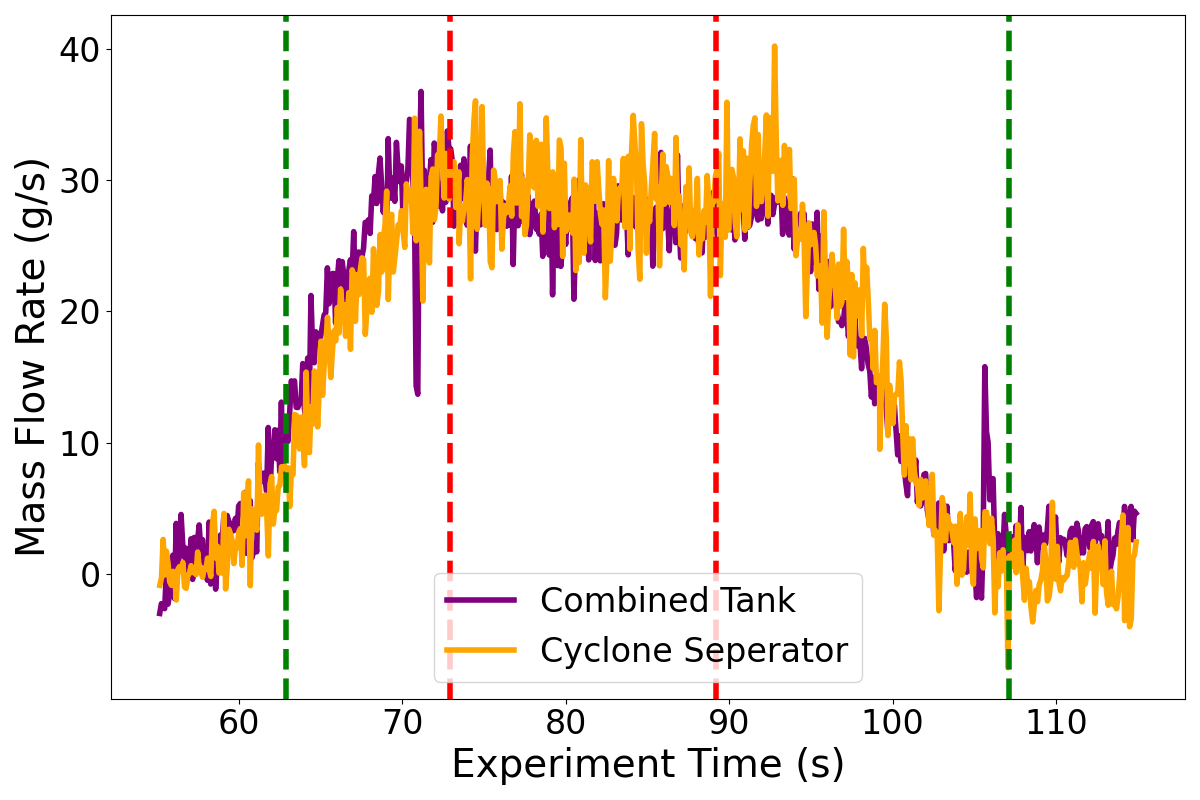
\includegraphics[width=\textwidth]{../report_assets/43_clean_flow_100.png}
        \caption*{Mass Flow Rate with 100 smoothing.}
    \end{minipage}
    \caption{3rd Test 4 Bar Inlet}
    
\end{figure}\label{fig:43}
\newpage
\begin{figure}[htbp]
    \centering

    \begin{minipage}{0.3\textwidth}
        \centering
        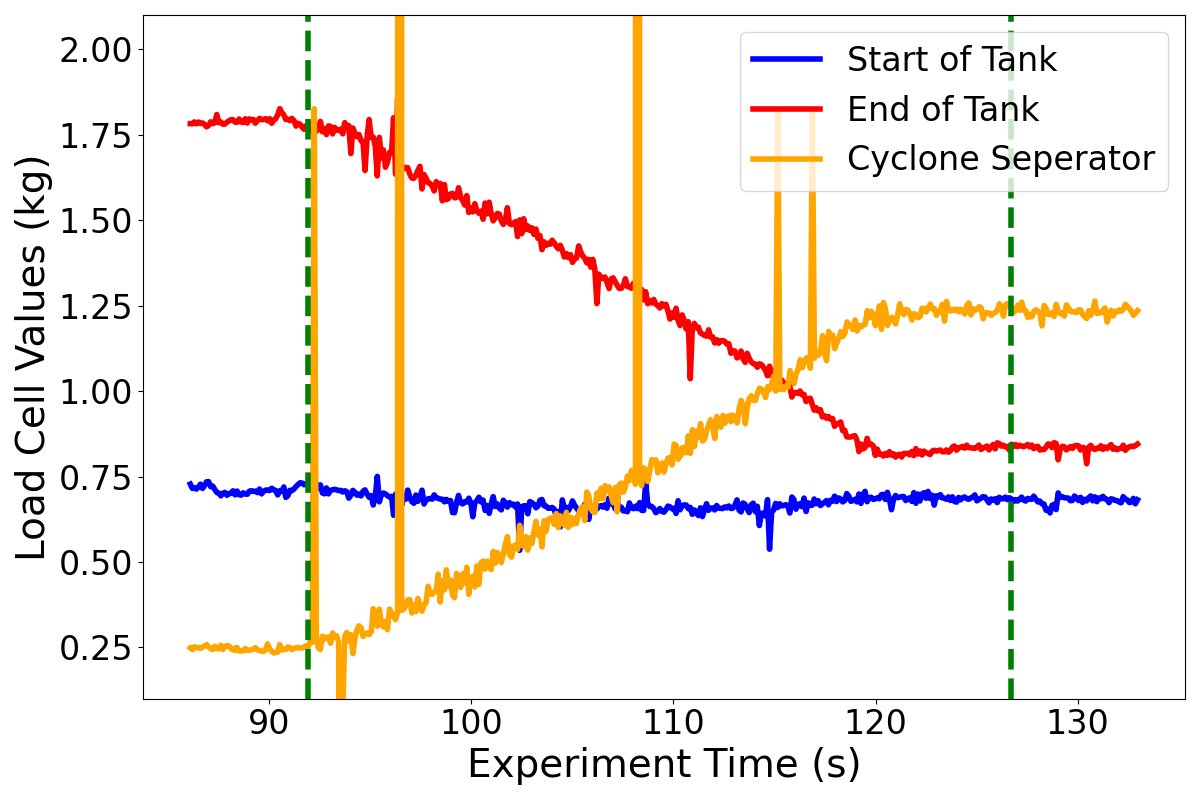
\includegraphics[width=\textwidth]{../report_assets/51_raw_mass.png}
        \caption*{Raw Load Cell Readings.}
    \end{minipage}
    \hfill
    \begin{minipage}{0.3\textwidth}
        \centering
        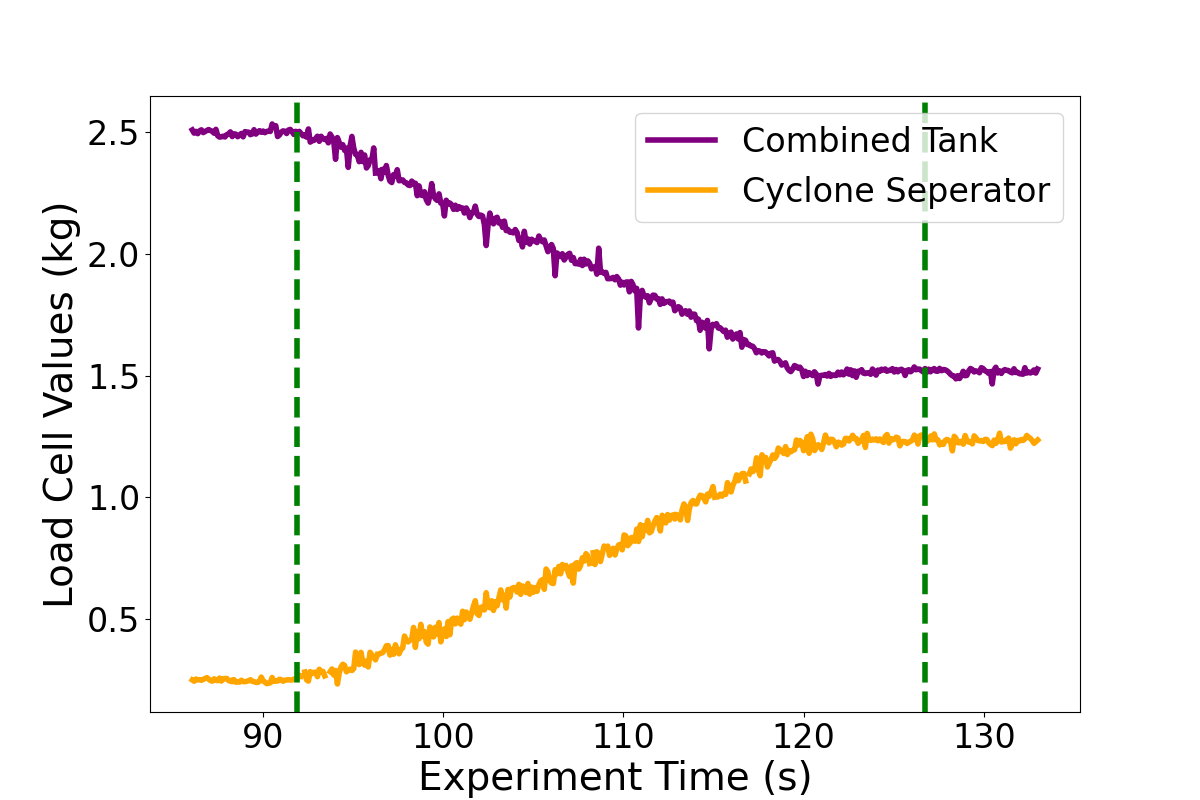
\includegraphics[width=\textwidth]{../report_assets/51_clean_mass.png}
        \caption*{Cleaned Mass Change.}
    \end{minipage}
    \hfill
    \begin{minipage}{0.3\textwidth}
        \centering
        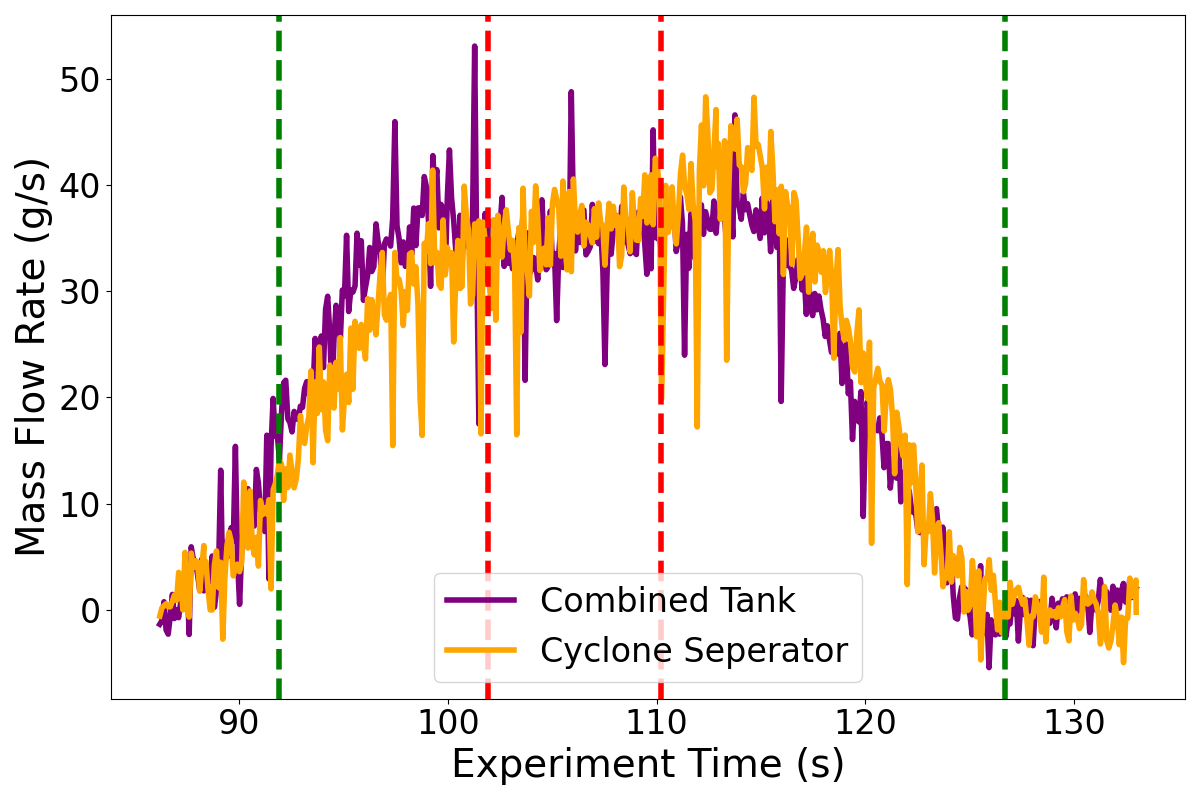
\includegraphics[width=\textwidth]{../report_assets/51_clean_flow_100.png}
        \caption*{Mass Flow Rate with 100 smoothing.}
    \end{minipage}
    \caption{1st Test 5 Bar Inlet}
    
\end{figure}\label{fig:51}

\begin{figure}[htbp]
    \centering

    \begin{minipage}{0.3\textwidth}
        \centering
        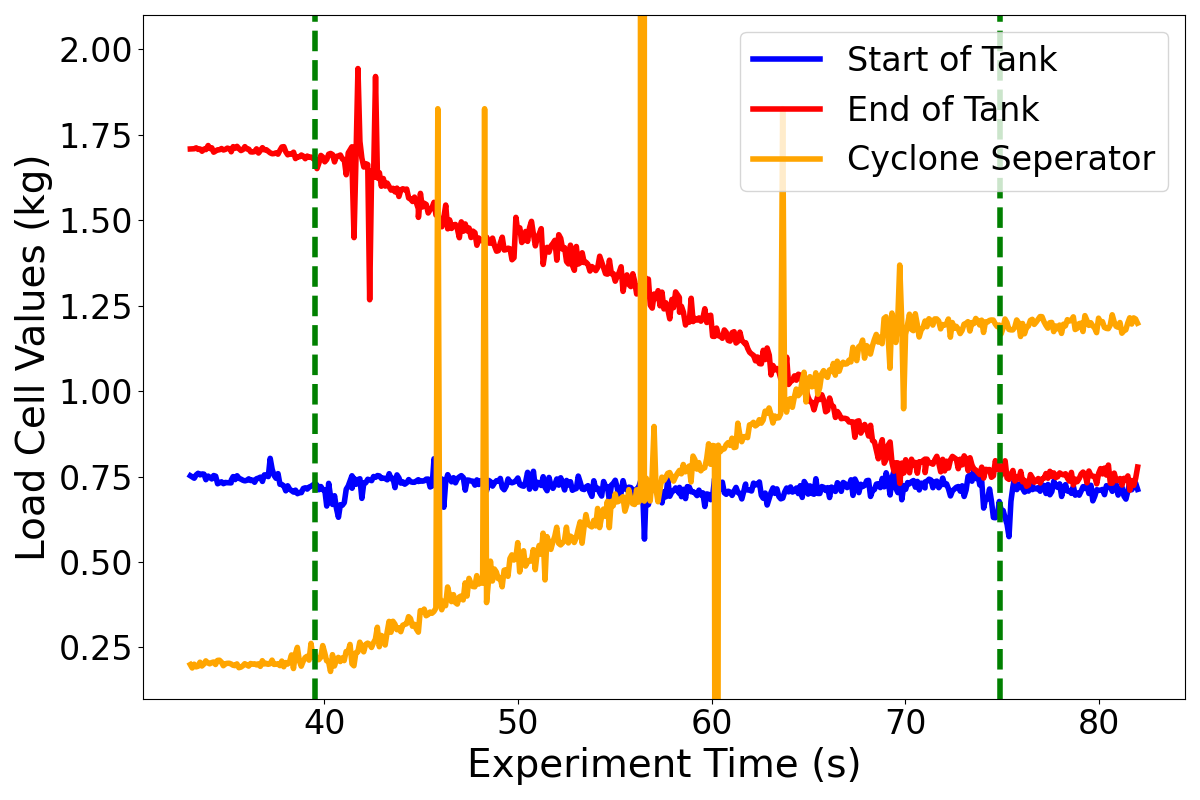
\includegraphics[width=\textwidth]{../report_assets/52_raw_mass.png}
        \caption*{Raw Load Cell Readings.}
    \end{minipage}
    \hfill
    \begin{minipage}{0.3\textwidth}
        \centering
        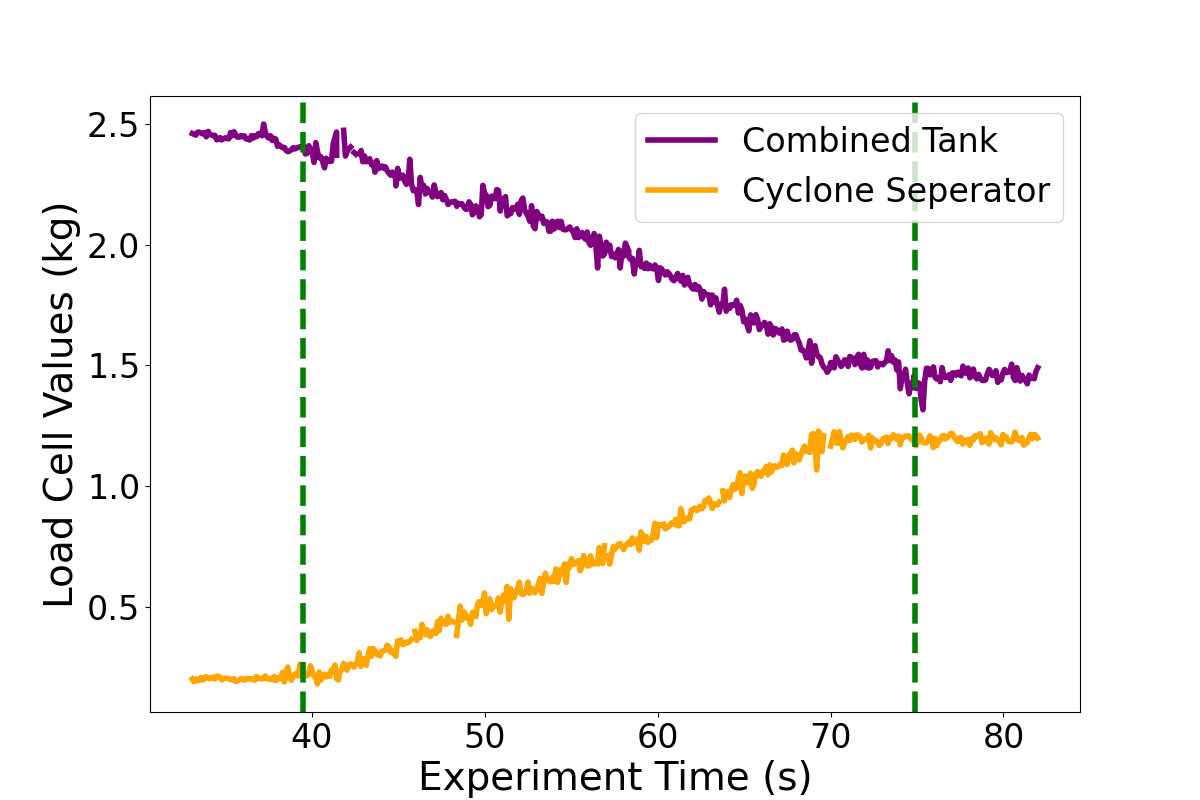
\includegraphics[width=\textwidth]{../report_assets/52_clean_mass.png}
        \caption*{Cleaned Mass Change.}
    \end{minipage}
    \hfill
    \begin{minipage}{0.3\textwidth}
        \centering
        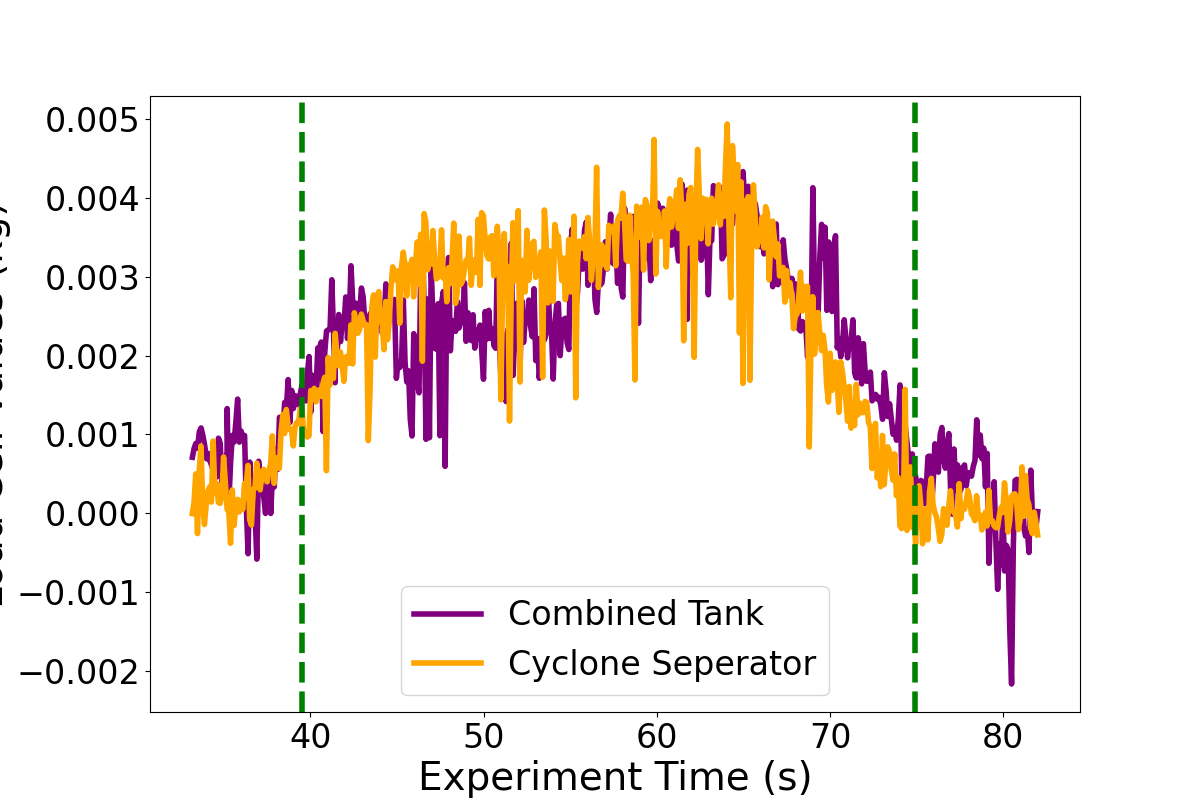
\includegraphics[width=\textwidth]{../report_assets/52_clean_flow_100.png}
        \caption*{Mass Flow Rate with 100 smoothing.}
    \end{minipage}
    \caption{1st Test 5 Bar Inlet}
    
\end{figure}\label{fig:52}

\begin{figure}[htbp]
    \centering

    \begin{minipage}{0.3\textwidth}
        \centering
        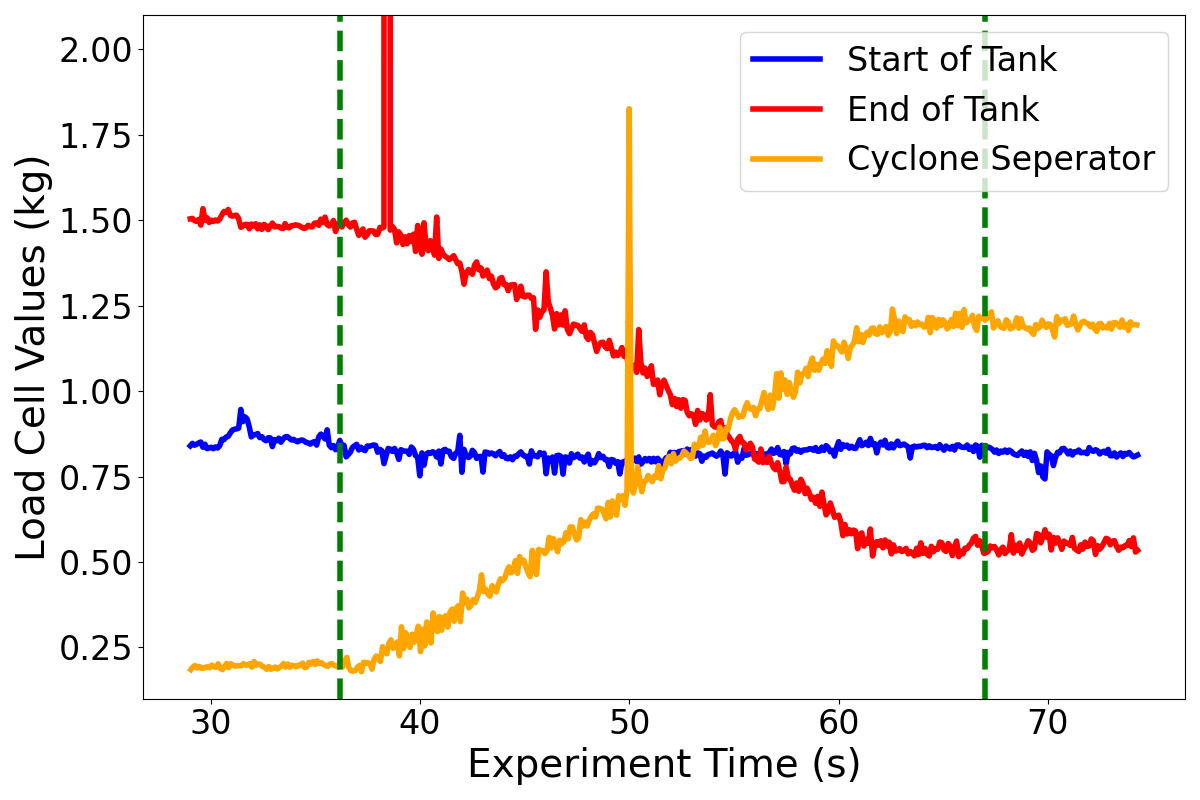
\includegraphics[width=\textwidth]{../report_assets/53_raw_mass.png}
        \caption*{Raw Load Cell Readings.}
    \end{minipage}
    \hfill
    \begin{minipage}{0.3\textwidth}
        \centering
        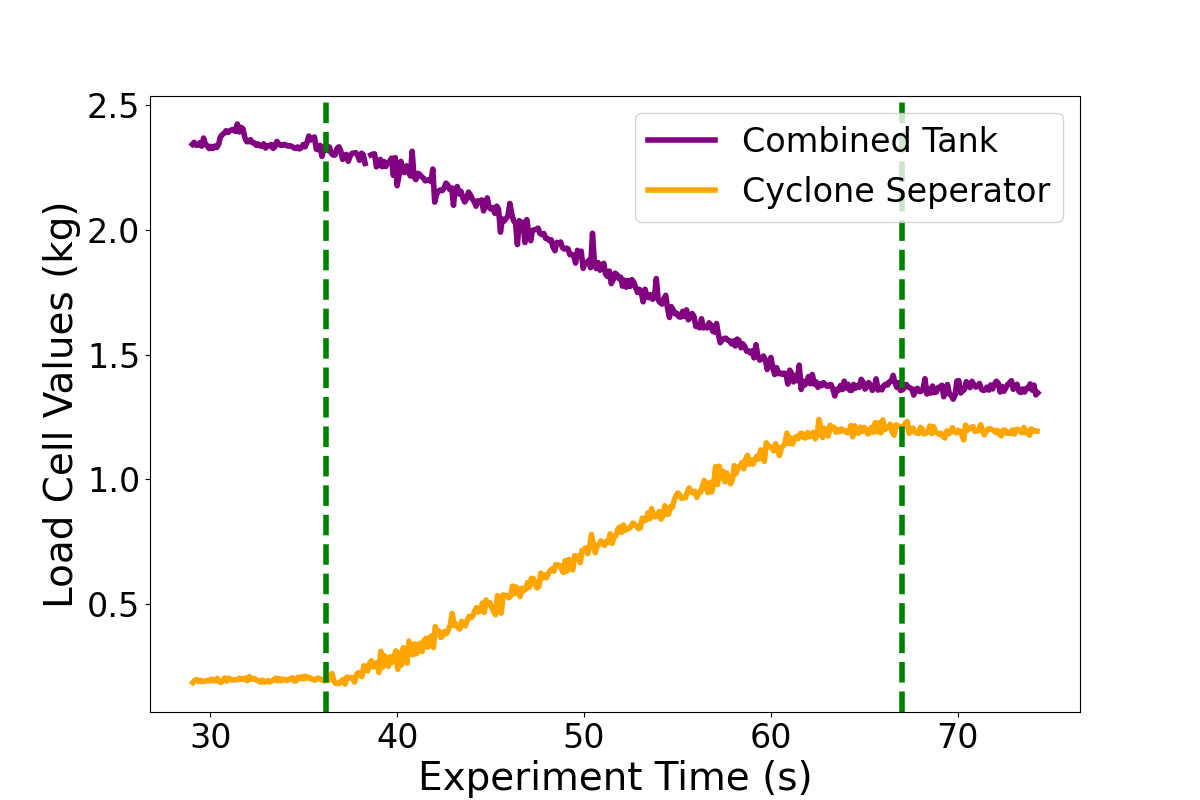
\includegraphics[width=\textwidth]{../report_assets/53_clean_mass.png}
        \caption*{Cleaned Mass Change.}
    \end{minipage}
    \hfill
    \begin{minipage}{0.3\textwidth}
        \centering
        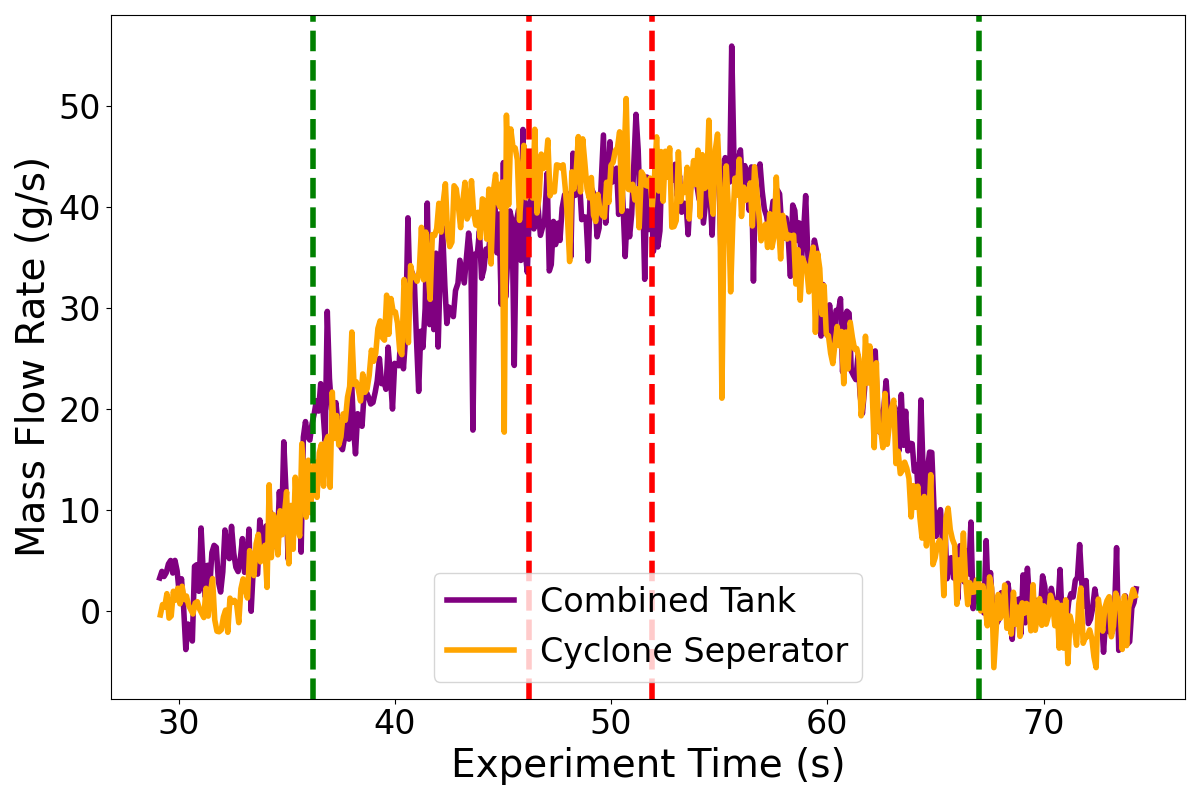
\includegraphics[width=\textwidth]{../report_assets/53_clean_flow_100.png}
        \caption*{Mass Flow Rate with 100 smoothing.}
    \end{minipage}
    \caption{1st Test 5 Bar Inlet}
    
\end{figure}\label{fig:53}

While each invidual test well endorses the system, especially 3rd test 4 bar, due to the reliable and high mass flow rate, repeatability is severly lacking.

It was expected that higher pressures would have smoothed out the flow rate as ??? when in reality it only increased the issue. 